\documentclass[12pt]{report}

% includes
\usepackage{listings}           % for inline code
\usepackage{geometry}           % page size
\usepackage[utf8]{inputenc}     % encoding
\usepackage{palatino}           % font
\usepackage[english]{babel}     % language
\usepackage{graphicx}           % images
\usepackage{indentfirst}        % indentation
\usepackage[nottoc]{tocbibind}  % table of contents style
\usepackage[unicode]{hyperref}  % references from the table of contents
\usepackage{xcolor}             % to define colors


% includes options
\geometry{  a4paper,            % scientific thesis standard
            left=3cm,
            right=2cm,
            top=2cm,
            bottom=2cm,
 }
\graphicspath{{images/}}        % path where the images are located
\setlength{\parindent}{1cm}     % paragraph indentation

% other options
\linespread{1.5}                % space between lines
\renewcommand*\contentsname{Cuprins}    % table of contents name

\setlength{\parindent}{1cm}     % paragraph indentation

\definecolor{codegreen}{rgb}{0,0.6,0}
\definecolor{codegray}{rgb}{0.5,0.5,0.5}
\definecolor{codepurple}{rgb}{0.58,0,0.82}
\definecolor{backcolour}{rgb}{0.95,0.95,0.92}
\lstdefinestyle{mystyle}{
    backgroundcolor=\color{backcolour},   
    commentstyle=\color{codegreen},
    keywordstyle=\color{magenta},
    numberstyle=\tiny\color{codegray},
    stringstyle=\color{codepurple},
    basicstyle=\ttfamily\footnotesize,
    breakatwhitespace=false,         
    breaklines=true,                 
    captionpos=b,                    
    keepspaces=true,                 
    numbers=left,                    
    numbersep=5pt,                  
    showspaces=false,                
    showstringspaces=false,
    showtabs=false,                  
    tabsize=2
}
\lstset{style=mystyle}


% the document content
\begin{document}
    % macros (global)
    \newcommand{\university}    {"Alexandru-Ioan Cuza" University, Iași}
\newcommand{\universityg}   {"Alexandru-Ioan Cuza" University, Iași} % genitive
\newcommand{\faculty}       {Faculty of Computer Science}
\newcommand{\facultyg}      {Faculty of Computer Science} % genitive
\newcommand{\speciality}    {computer science}
\newcommand{\promotion}     {2022}                                  %<---------

\newcommand{\thesistype}    {Master's Thesis}
\newcommand{\thesistitle}   {Solidity Optimization using Control Flow Graphs}    %<---------

\newcommand{\authorlast}    {Iacob}                               %<---------
\newcommand{\authorfirst}   {Sergiu}
\newcommand{\authornamefl}  {\authorfirst \space \authorlast} % first name first
\newcommand{\authornamelf}  {\authorlast \space \authorfirst} % last name first
\newcommand{\authorbirth}   {01 March 1997}                      %<---------
\newcommand{\authoraddress} {România, jud. Iași, mun. Iași} %<---------
\newcommand{\authorcnp}     {-}                         %<---------

\newcommand{\session}       {july, 2022}                       %<---------
\newcommand{\coordinator}   {Dr. Arusoaie Andrei}               %<---------

\newcommand{\dottedline}    {............................}
    
    % front-matter
    \pagenumbering{gobble}
    
    % define the cover page
\begin{titlepage}
    \begin{center}
        % the university and faculty
        \large
        \MakeUppercase{\university}
        
        \LARGE
        \textbf{\MakeUppercase{\faculty}}
        
        % the faculty logo
        \vspace{1cm}
        
\includegraphics[width=0.3\textwidth]{logoFii.png}
        
        % thesis title
        \vspace{1cm}
        \Large
        \MakeUppercase{\thesistype}
        
        \vspace{0.5cm}
        \LARGE
        \textbf{\thesistitle}
        
        % author
        \vspace{2cm}
        \Large
        proposed by
        
        \vspace{0.5cm}
        \LARGE
        \textbf{\authornamelf}
        
        % session
        \vfill
        \Large
        \textbf{Session:} \session
        
        % scientific coordinator
        \vspace{2cm}
        \Large
        Scientific Coordinator
        
        \vspace{0.5cm}
        \LARGE
        \textbf{\coordinator}
    \end{center}
\end{titlepage}
    % define the title page
\begin{titlepage}
    \begin{center}
        % the university and faculty
        \large
        \MakeUppercase{\university}
        
        \LARGE
        \textbf{\MakeUppercase{\faculty}}
        
        % thesis title
        \vspace{8cm}
        \huge
        \textbf{\thesistitle}
        
        % author
        \vspace{2cm}
        \LARGE
        \textbf{\authornamefl}
        
        % session
        \vfill
        \Large
        \textbf{Session:} \session
        
        % scientific coordinator
        \vspace{4cm}
        \Large
        Coordinator
        
        \vspace{0.5cm}
        \LARGE
        \textbf{\coordinator}
    \end{center}
\end{titlepage}
    % \vspace*{\fill}

\begin{flushright}
    Avizat, \\
    Îndrumător lucrare de licență, \\
    \coordinator. \\
    Data: \dottedline \hspace{1cm} Semnătura: \dottedline
\end{flushright}

\vspace{1cm}
\begin{center}
    \large
    \textbf{Declarație privind originalitatea conținutului lucrării de licență}
\end{center}

Subsemnatul \textbf{\authornamelf} domiciliat în \textbf{\authoraddress}, născut la data de \textbf{\authorbirth}, identificat prin CNP \textbf{\authorcnp}, absolvent al \facultyg, \textbf{\faculty} specializarea \textbf{\speciality}, promoția \promotion, declar pe propria răspundere cunoscând consecințele falsului în declarații în sensul art. 326 din Noul Cod Penal și dispozițiile Legii Educației Naționale nr. 1/2011 art. 143 al. 4 și 5 referitoare la plagiat, că lucrarea de licență cu titlul \textbf{\thesistitle} elaborată sub îndrumarea domnului \textbf{\coordinator}, pe care urmează să o susțin în fața comisiei este originală, îmi aparține și îmi asum conținutul său în întregime.

De asemenea, declar că sunt de acord ca lucrarea mea de licență să fie verificată prin orice modalitate legală pentru confirmarea originalității, consimțind inclusiv la introducerea conținutului ei într-o bază de date în acest scop.

Am luat la cunoștință despre faptul că este interzisă comercializarea de lucrări științifice în vederea facilitării falsificării de către cumpărător a calității de autor al unei lucrări de licență, de diplomă sau de disertație și în acest sens, declar pe proprie răspundere că lucrarea de față nu a fost copiată ci reprezintă rodul cercetării pe care am întreprins-o.

\begin{flushright}
    Data: \dottedline \hspace{6cm} Semnătura: \dottedline
\end{flushright}

\vspace*{\fill}
\pagebreak
    % \vspace*{\fill}
\begin{center}
    \large
    \textbf{Declarație de consimțământ}
\end{center}

Prin prezenta declar că sunt de acord ca lucrarea de licență cu titlul \textbf{\thesistitle}, codul sursă al programelor și celelalte conținuturi (grafice, multimedia, date de test, etc.) care însoțesc această lucrare să fie utilizate în cadrul \facultyg.

De asemenea, sunt de acord ca \faculty \space de la \university, să utilizeze, modifice, reproducă și să distribuie în scopuri necomerciale programele-calculator, format executabil și sursă, realizate de mine în cadrul prezentei lucrări de licență.

\begin{flushright}
    Absolvent \textbf{\authornamefl} \\
    \vspace{0.5cm}
    Data: \dottedline \hspace{6cm} Semnătura: \dottedline
\end{flushright}
\vspace*{\fill}
\pagebreak
    
    % table of contents
    \tableofcontents
    
    \cleardoublepage
    % \phantomsection
    \addcontentsline{toc}{chapter}{\listfigurename}
    \listoffigures
    
    % chapters
    \setcounter{page}{1}
    \pagenumbering{arabic}
    
    \chapter*{Motivation} 
\addcontentsline{toc}{chapter}{Motivation}

Blockchain has seen an increased popularity over the last few years. With more and more decentralized, scalable applications in the cloud, the software engineering industry has also seen an increase in blockchain development requests. It is futile to deny the revolutionary aspects of the Blockchain network, as it is usually the case with many new technologies in the market.

One of the keys for great software engineering is working with great, efficient tools – that is, the better, faster, more secure a programming language is, the better the final product is. In this thesis, we'll explore on how we can make Solidity, a programming language for developing smart contracts on the Blockchain, more efficient in building its bytecode and deploying the smart contracts in the network.

By the means of this work, we expect to see small improvements in the static analysis and compilation of the code, which in the end, multiplied by the hundreds of thousands of smart contracts compiled daily, might result in huge cost savings in the cloud.


    % \chapter{Introduction} 
\section{Context}
\paragraph*{}
Static analysis has been at the core of \textbf{optimizing} code for many years now, doubled by its sibling, dynamic analysis. Common programming languages such as C++, Java, Golang etc. generate \textbf{bytecode}, by the usage of \textbf{compilers}, that is eventually interpreted by various virtual machines, such as LLVM, on various architectures \textemdash \ x86, x86\_64, AMD64, arm64 etc.

\paragraph*{}
While the virtual machines that run bytecode and the cpu architectures are shared across programming languages, since they ultimately revolve around the same assembly instructions, each programming language has its own compiler while, of course, interpreted languages such as Python have their own interpreter.

\paragraph*{}
Zooming in on how a compiler works, we find the optimizer, which is a sort of Maslow pyramid level, but in the compiler world. While any compiled code may run just fine without it being optimized, it will more than likely miss on many performance improvements that will greatly speed up the code's run time and resources' usage.

\paragraph*{}
Writing high level code greatly simplifies the development process of software applications. It saves a lot of time, as writing low level code such as assembly often means a great deal of work, but necessary in some situations such as embedded software. Developers cannot always invest the needed time and knowledge to perfectly optimize their code, nor can they make a cpu's frequency higher by writing a line of code. What the compiler can do, instead, is less. Running less instructions, in a better order, using registers more efficiently and moving less memory blocks around is what gets us the fastest computation. This is ultimately the optimizer's job in a compiler \textemdash \ find opportunities to generate more efficient bytecode.


\section{Objective}

\paragraph*{}
The purpose of this thesis is to research the techniques of applying static analysis on high level code, in order to obtain efficient bytecode, regardless of the virtual machine it will execute on. These techniques are usually backed up by \textbf{intermediate representations} of the initial code, which can be either another high level code (with different syntax, but the same semantics), or data structures meant to provide an overview (or in-depth view) over the program execution.

\paragraph*{}
In this thesis, we will see how intermediate representations help, why they're useful, and how \textbf{Control Flow Graphs} determine which optimizations can be applied while doing static analysis. The programming language we will focus on is \textbf{Solidity} \footnote{Solidity is a highly volatile language at this point, therefore it is probable that some of the details presented in this thesis will lose veridicity in the near future. However, the high-level schemas, approaches and structure of the Solidity eco-system will likely remain the same.}.

\section{Motivation}

\paragraph*{}
Solidity is a new programming language on the market, backing up the development of Smart Contracts mostly deployed on the Ethereum blockchain. Since it is a relatively new technology, there is a lot of ongoing work to still build the basis of the eco-system and to enhance the compiler by basic features or common optimizations.

\paragraph*{}
An important aspect is that Solidity is an open-source technology, which facilitates \textbf{external contributions}, some of which will be provided by the usage of this thesis. Optimization sits at the heart of the compiler, and as the official documentation states, \cite[the optimizer is under heavy development]{solidity-yul-optimizer}. This is sufficiently encouraging to research on how Control Flow Graphs, intermediate representations and static analysis techniques could be combined in order to improve the bytecode generated from Solidity.

\section{Thesis structure}
\paragraph*{}
Bringing external contributions to a technology usually follows a logical timeline, around which this thesis was also structured. Specifically in our case, we'll go through understanding Solidity and its usecases, understanding what a compiler and what a optimizer is, how Solidity's compiler works, what are some of its optimizer's drawbacks and how we should solve these. Finally, we go through integrating our improvements into the actual Solidity codebase.

\paragraph*{}
In the first chapters, we set the knowledge base needed to improve the optimizer. We go through Solidity and the (relatively) new Yul IR, static analysis, control flow graphs (CFG), abstract syntax trees (AST) and the Solidity optimizer structure.

\paragraph*{}
In the latter chapters, we do a deep dive into a few optimization steps and identify edge cases not optimized by these and do a few benchmarks to see how much gas is saved through these improvements. Finally, we conclude with some experiments on Etherscan, where we try to see if the enhancements have an impact on verified smart contracts.

    
    \chapter{Solidity}

\section{Overview}
\paragraph*{}
Solidity is a relatively new programming language, its first proposal coming in 2014 from the co-founder of Ethereum, Gavin Wood \cite{solidity-lang}. Its purpose is to serve development of smart contracts to be deployed on various blockchain platforms, especially focusing on the Ethereum blockchain.

\paragraph*{}
Although it's been around for around 8 years now, Solidity has just started to peak interest in the blockchain development community. Dune Analytics reported an increase of 75\% in smart contracts deployment in March, 2020, summing up to a total of 2 million smart contracts deployed \cite{coin-telegraph-2020}. Since then, hundreds of thousands of smart contracts have been deployed monthly, with around 370 thousands just in May 2022 \ref{fig:dune-analytics-2022}.

\begin{figure}
    \centering
    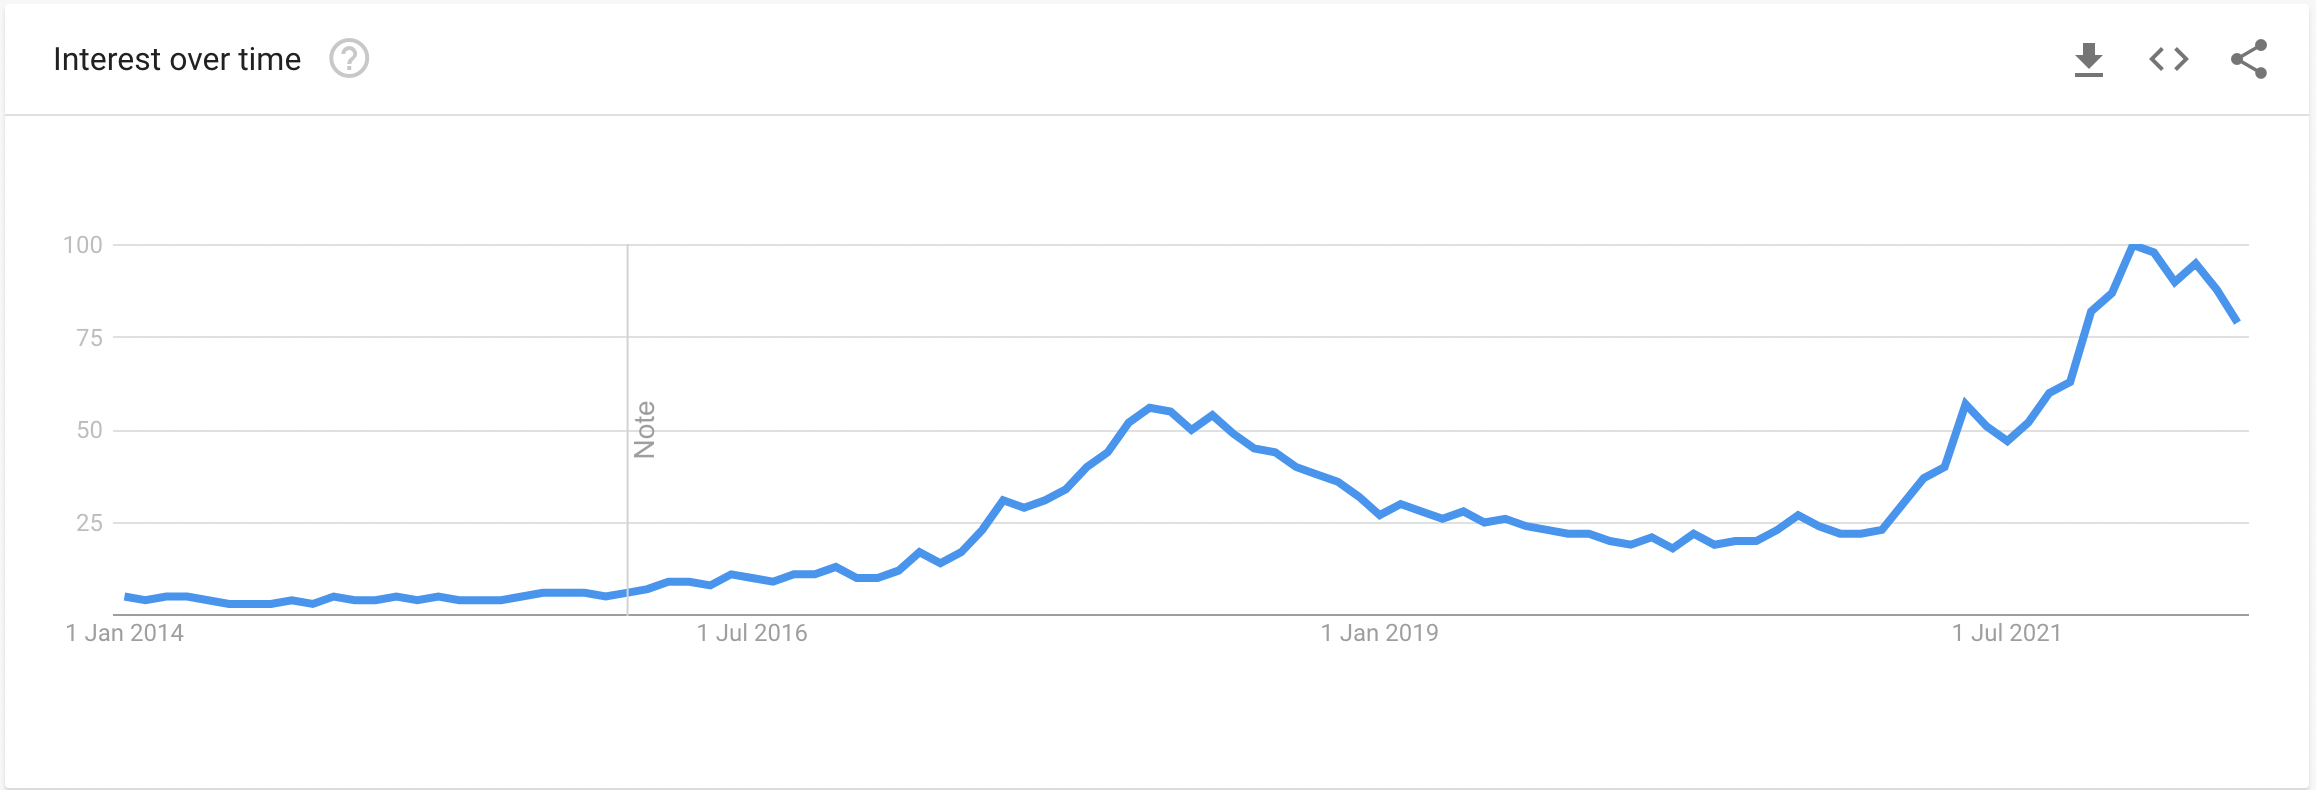
\includegraphics[width=15cm]{images/solidity_interest.png}
    \caption{Solidity interest from 1st of January, 2014, to 1st of June, 2022, according to Google web searches}
    \label{fig:solidity-interest}
\end{figure}

\begin{figure}
    \centering
    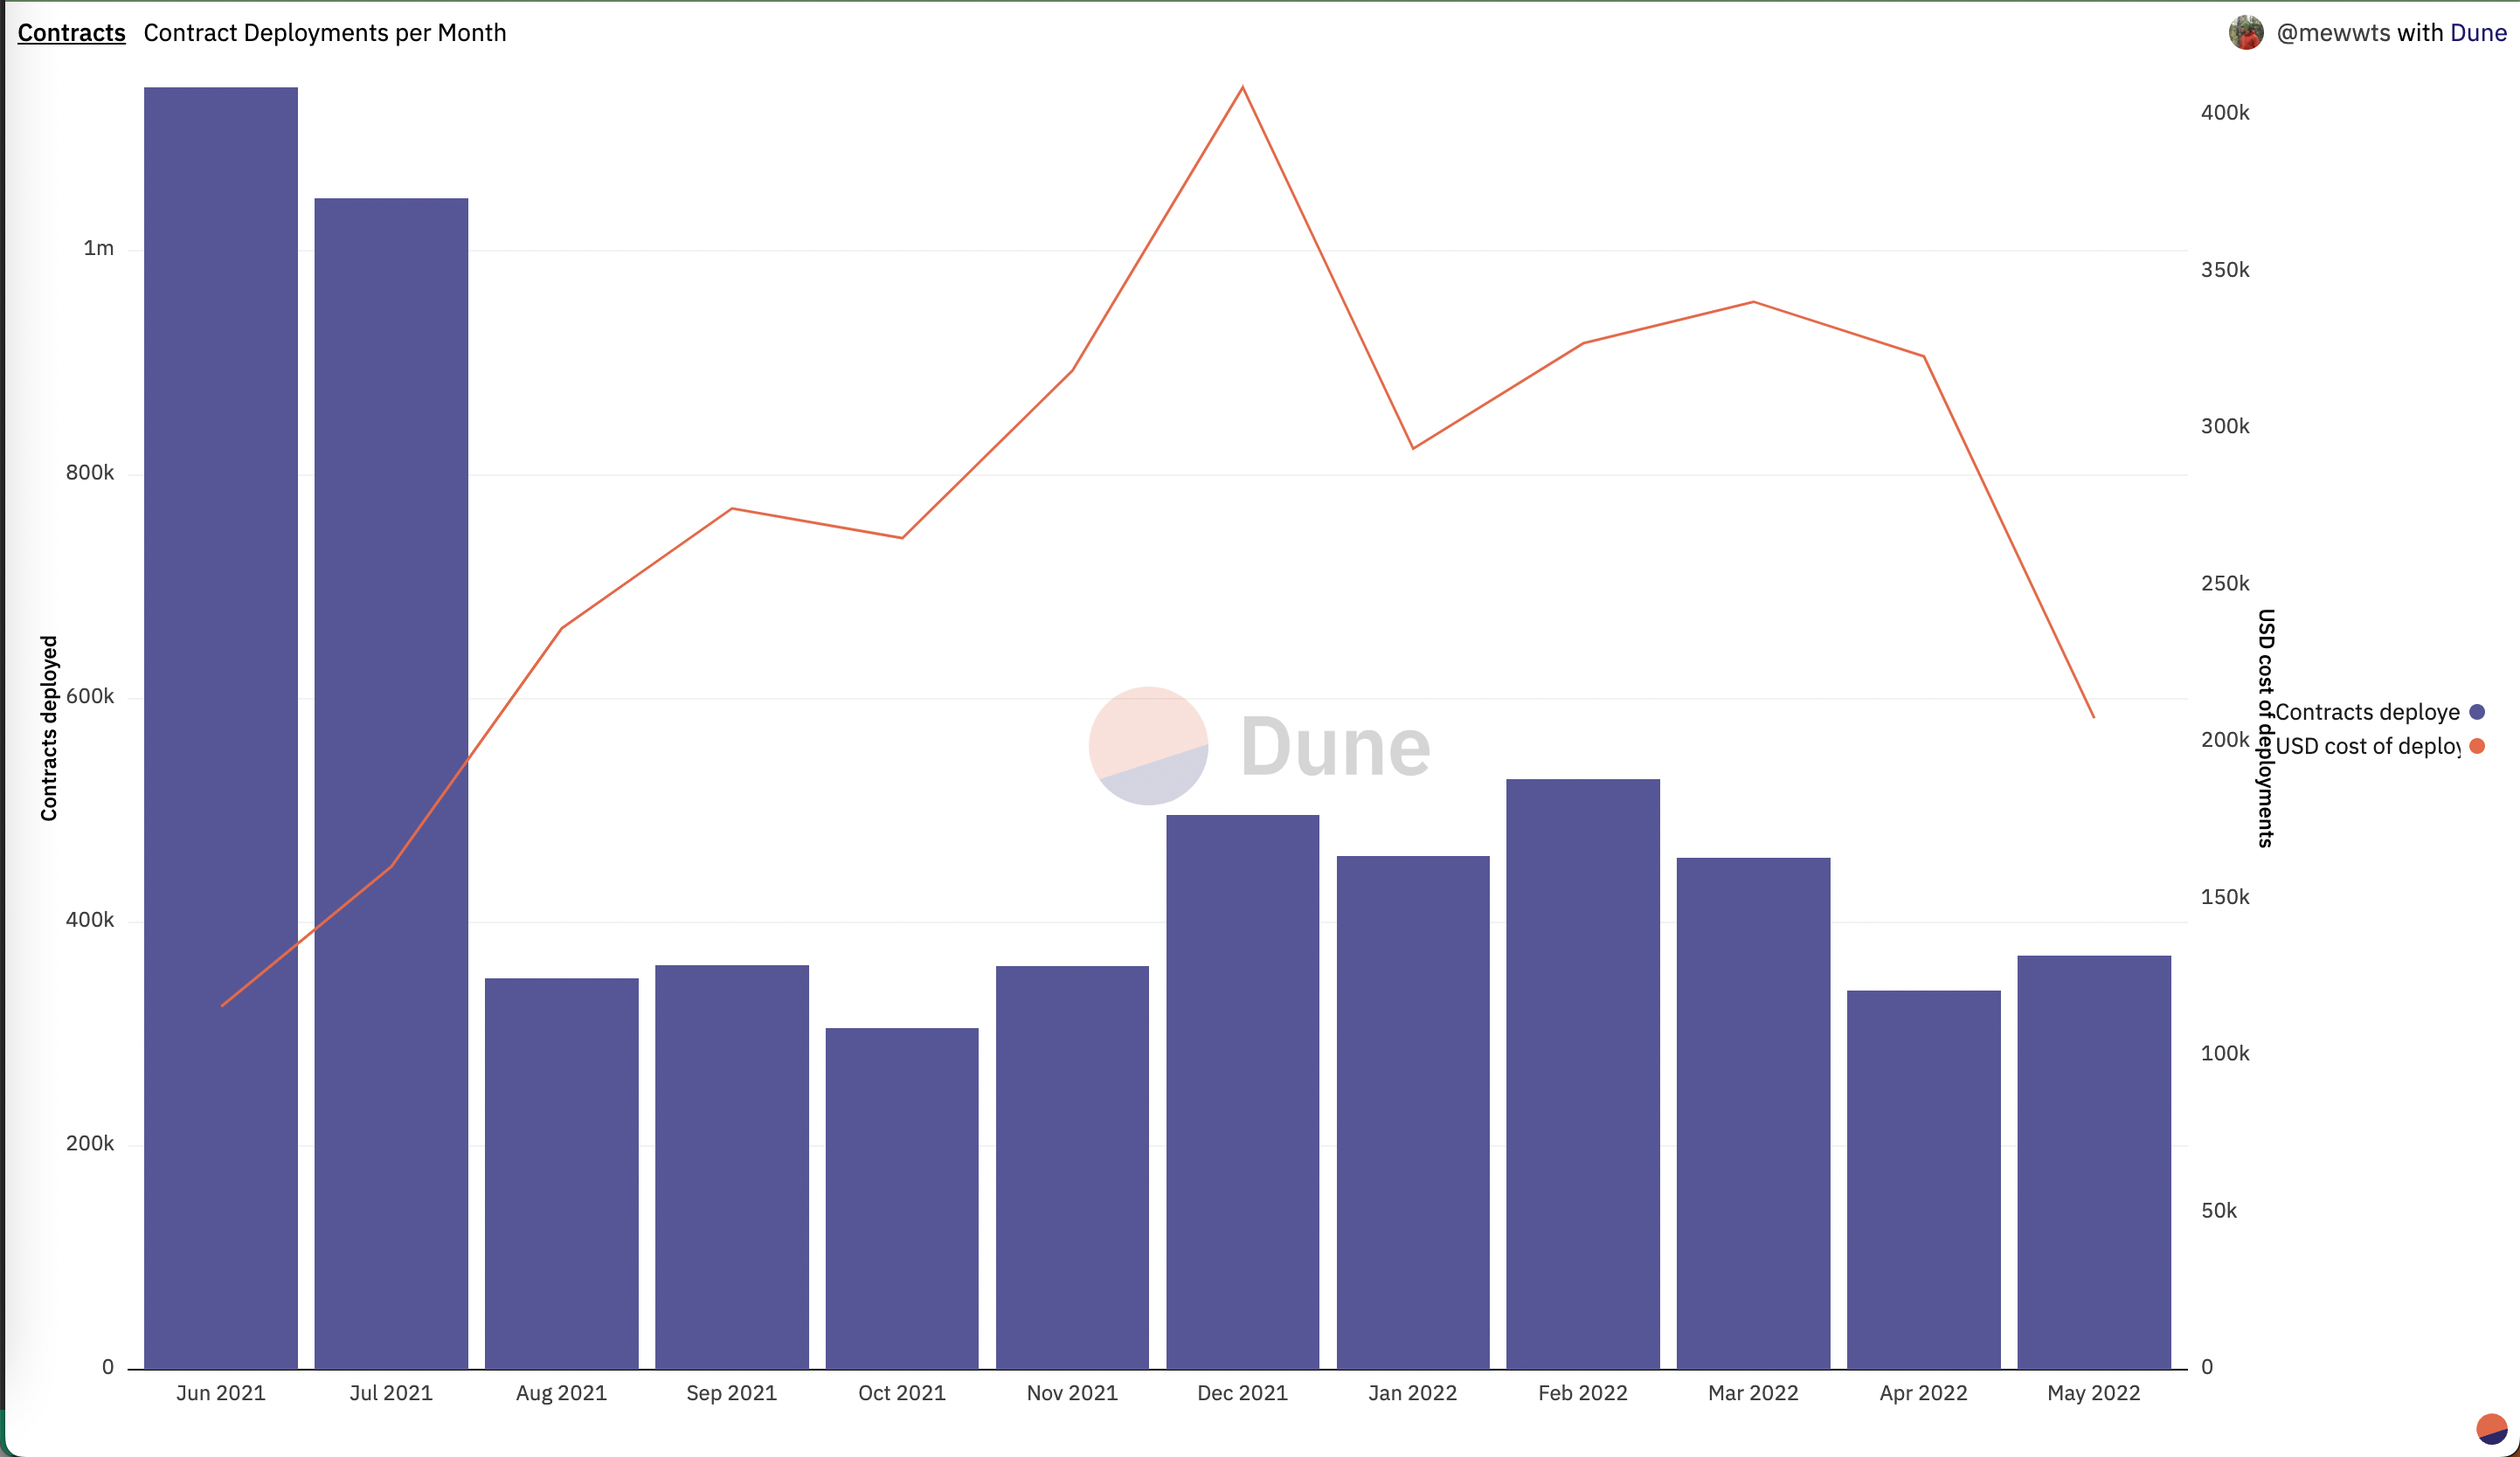
\includegraphics[width=15cm]{images/dune_analytics_2022.png}
    \caption{Contract deployment per month in the past year, according to Dune Analytics}
    \label{fig:dune-analytics-2022}
\end{figure}

\paragraph*{}
The main properties that interests this thesis are that this programming language is \textbf{statically typed} and is converted into bytecode to run inside the Ethereum Virtual Machine (EVM). Being statically typed helps the compiler with static analysis, making possible the development of an optimization suite that performs both common optimizations and particular optimizations for EVM.

\section{Solidity's Compiler and Optimizer}
\paragraph*{}
High level solidity code is sent to \lstinline[columns=fixed]{solc} binary, which stands for ``solidity compiler''. The user may or may not specify the usage of the optimizer with the \lstinline[columns=fixed]{--optimize} flag, which is enabled by default. Upon analyzing the compilation flow \ref*{fig:solc-compilation-flow}, we notice that there are some optional (yet recommended) steps to follow while compiling, which take advantage of Yul (intermediate code representation for Solidity) and Abstract Syntax Trees, the latter being built for both the initial Solidity code and for the Yul IR. If we choose to optimize the code through Yul, then the \lstinline[columns=fixed]{--via-ir} must be specified, which is also enabled by default.

\paragraph*{}
When optimizing through Yul, the compilation flow will actually use \textbf{two optimizers}: the "new" one (Yul optimizer) and the "legacy" one (EVM bytecode optimizer). The reasoning behind this is that bytecode optimization should be as simple and straightforward as possible, this also being an engineering decision made by Solidity's team that they explained in the Solidity Summit presentations, 2022. \lstinline[columns=fixed]{JUMP} instructions are especially tricky to handle while optimizing bytecode, making high level, semantic optimization (for example simplifying \lstinline[columns=fixed]{for} loops) more difficult.

\paragraph*{}
The advantage of having two optimizers is that it decouples work by a great deal. Low level assembly optimizations are done by the legacy optimizer \footnote{Future work might also consist in unifying EVM and LLVM, bringing all of the work and optimization done to LLVM on Solidity's ground as well.}, and more complex optimizations, that require techniques such as data flow analysis, are done directly on the Yul IR, which is later used to generate the efficient bytecode. This also helps to visually inspect the generated Yul IR and making sure that its output is the expected one. Specifically for the team, it means that it makes unit testing and development much easier.

\begin{figure}
    \centering
    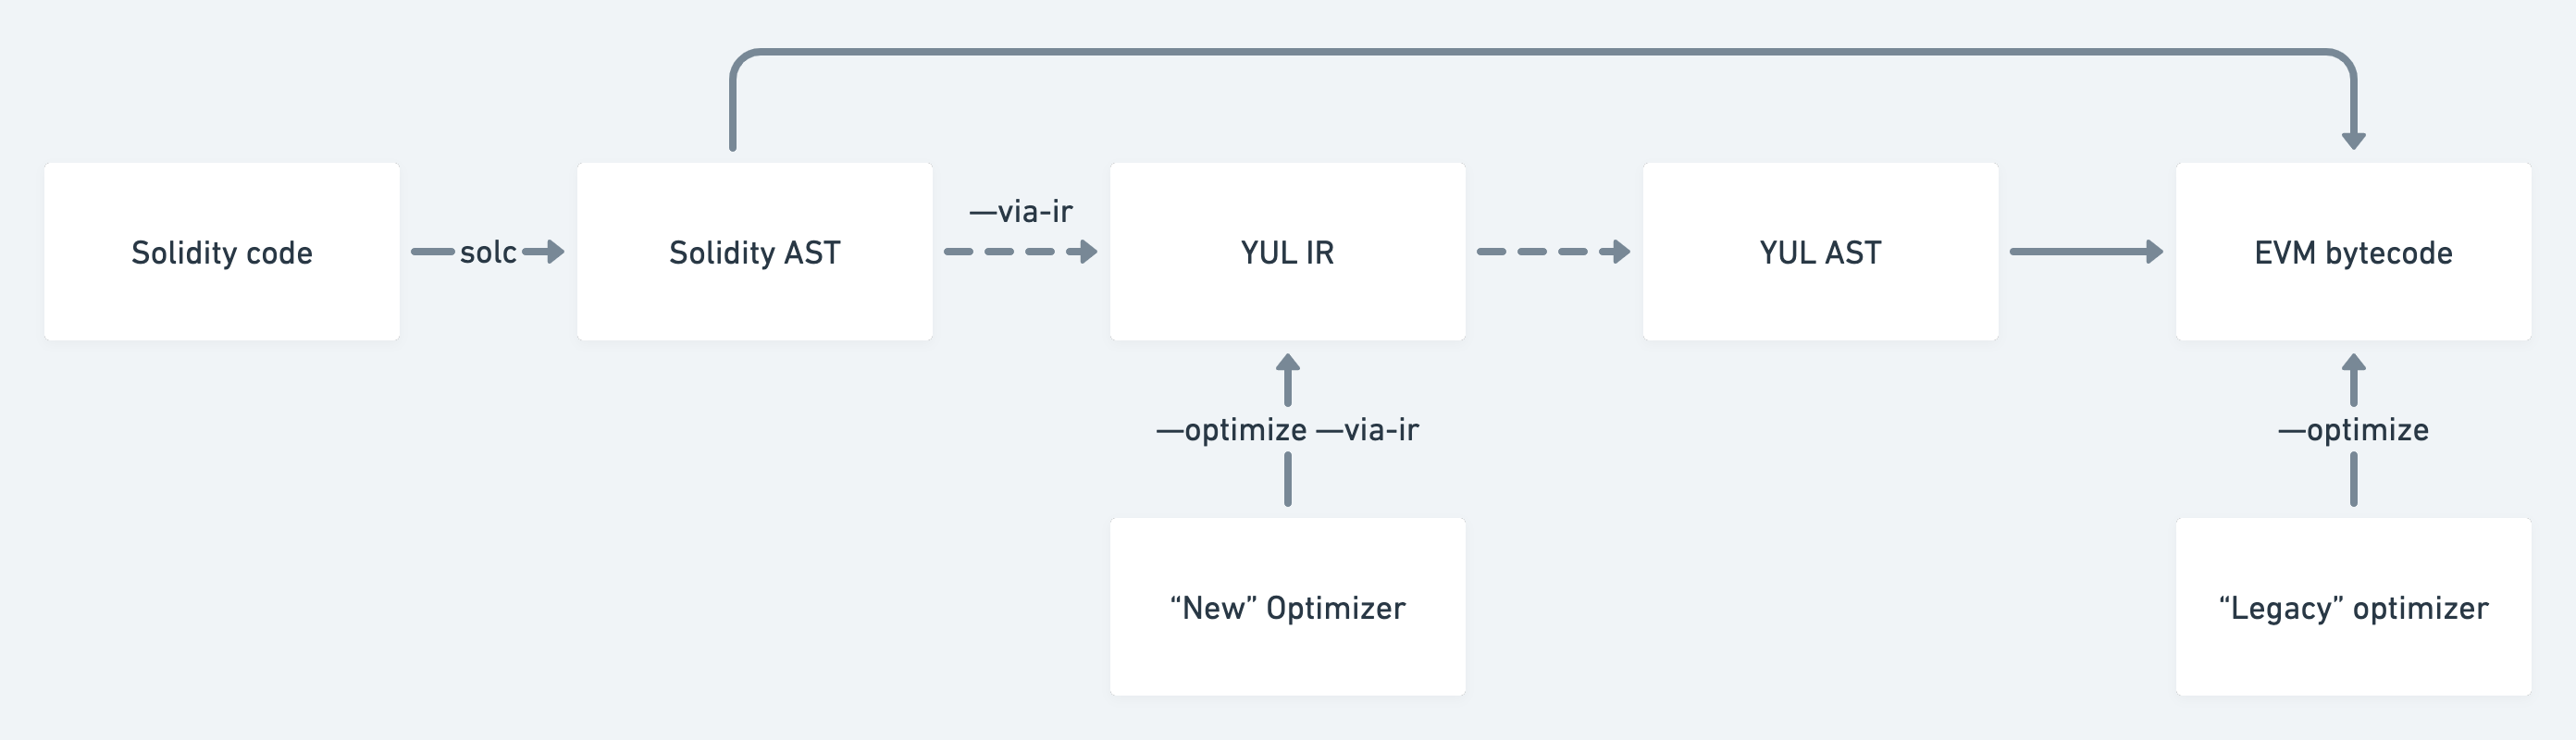
\includegraphics[width=15cm]{images/solc_flow.png}
    \caption{Solidity compilation flow}
    \label{fig:solc-compilation-flow}
\end{figure}

\section{Intermediate Representations}

\subsection*{Abstract Syntax Tree}
\paragraph*{}
\textbf{Abstract Syntax Trees (AST)} are often used to do a first analysis of the code instructions by walking the tree. This is often coupled with the Visitor Design Pattern, where the user implements what the \lstinline[columns=fixed]{visit} function should do for each type of node. They are often used in compilers to represent the structure of the code, to make isolated code changes and then re-generate code from the AST.

\paragraph*{}
Solidity uses ANTLR (ANother Tool for Language Recognition) to generate its AST. On Solidity's territory, ASTs appear in two phases. First, an AST is generated from the unaltered Solidity code, while another AST is later generated from the Yul IR code. The AST nodes provide sufficient granularity to make a structural analysis simple enough, thanks to recursively analysing the children node of a root.

\begin{figure}
    \centering
    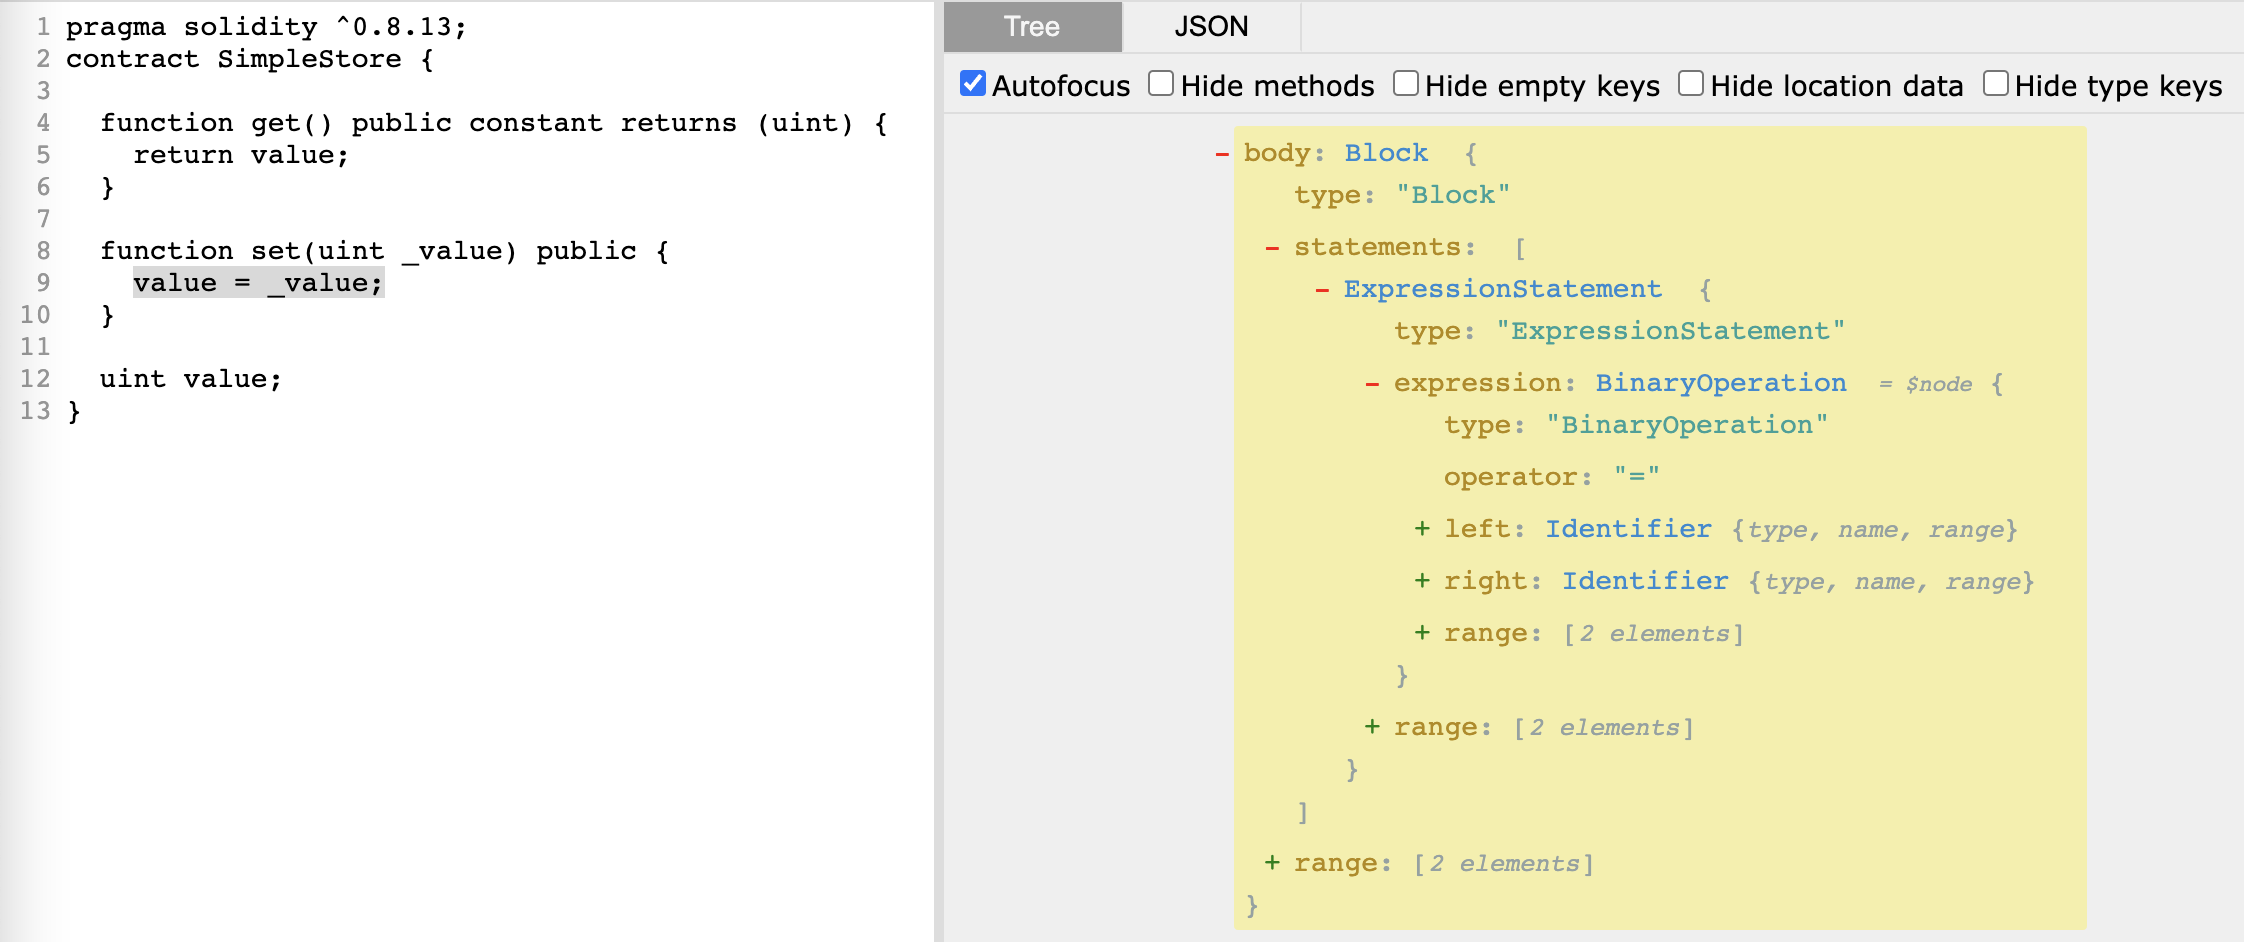
\includegraphics[width=15cm]{images/solidity_ast_example.png}
    \caption{Solidity AST Example. The body of the function is an AST node itself, in which the statements are other AST nodes. Generated using AST Explorer.}
    \label{fig:solidity-ast-example}
\end{figure}

\paragraph*{}
ASTs are very common in static analysis and are often times coupled with a grammar (or dialect) that enforces different node types and node structure in the tree. There are a variety of tools that use ASTs to do code analysis of their own.

% ASTs generated from Solidity code have been used by a variety of tools to inspect code, one of which is Solidity Instrumentation Framework (SIF) \ref{fig:sif-workflow}. The framework builds an internal representation (in C) of the AST nodes, bringing an additional set of features such as symbol renaming or function listing to the table. This works by exposing the \lstinline[columns=fixed]{visit} function to the user, each node being visited with the pattern implemented by the user.


\subsection*{Yul IR}
\paragraph*{}
\textbf{Yul}, former name Julia, is an intermediate representation for Solidity Code. It has been publicly announced as ``production ready'' in March, 2022, in version 0.8.13 of Solidity. Since then, the engineering team has been encouraging people to compile smart contracts via the usage of Yul, since the optimization focus has shifted on this pseudocode language.

\paragraph*{}
Yul was designed around four main principles, as described by its official documentation \cite{yul-description}: readability, easy manual inspection of control flow, simple and straightforward generation of bytecode from Yul and whole-program optimization. As compared to bytecode, this IR provides high-level syntax for instructions that introduce jump instructions (\lstinline[columns=fixed]{JUMP, JUMPDEST, JUMPI}), the reasoning behind this being that it makes analyzing data flow and control flow in the code much easier.

\begin{lstlisting}[caption={Example of Yul code which computes exponentiation recursively}]
{
    function power(base, exponent) -> result
    {
        switch exponent
        case 0 { result := 1 }
        case 1 { result := base }
        default
        {
            result := power(mul(base, base), div(exponent, 2))
            switch mod(exponent, 2)
                case 1 { result := mul(base, result) }
        }
    }
}
\end{lstlisting}

\paragraph*{}
This was designed as an actual programming language, making it possible to generate valid EVM bytecode from Yul code. Of course, it is not recommended to write smart contracts in Yul, but one can do so to get more familiar with the dialect. It also takes on the property of its "parent" code, and is also statically typed as Solidity. This further eases the static analysis done by the compiler.

\begin{figure}
    \centering
    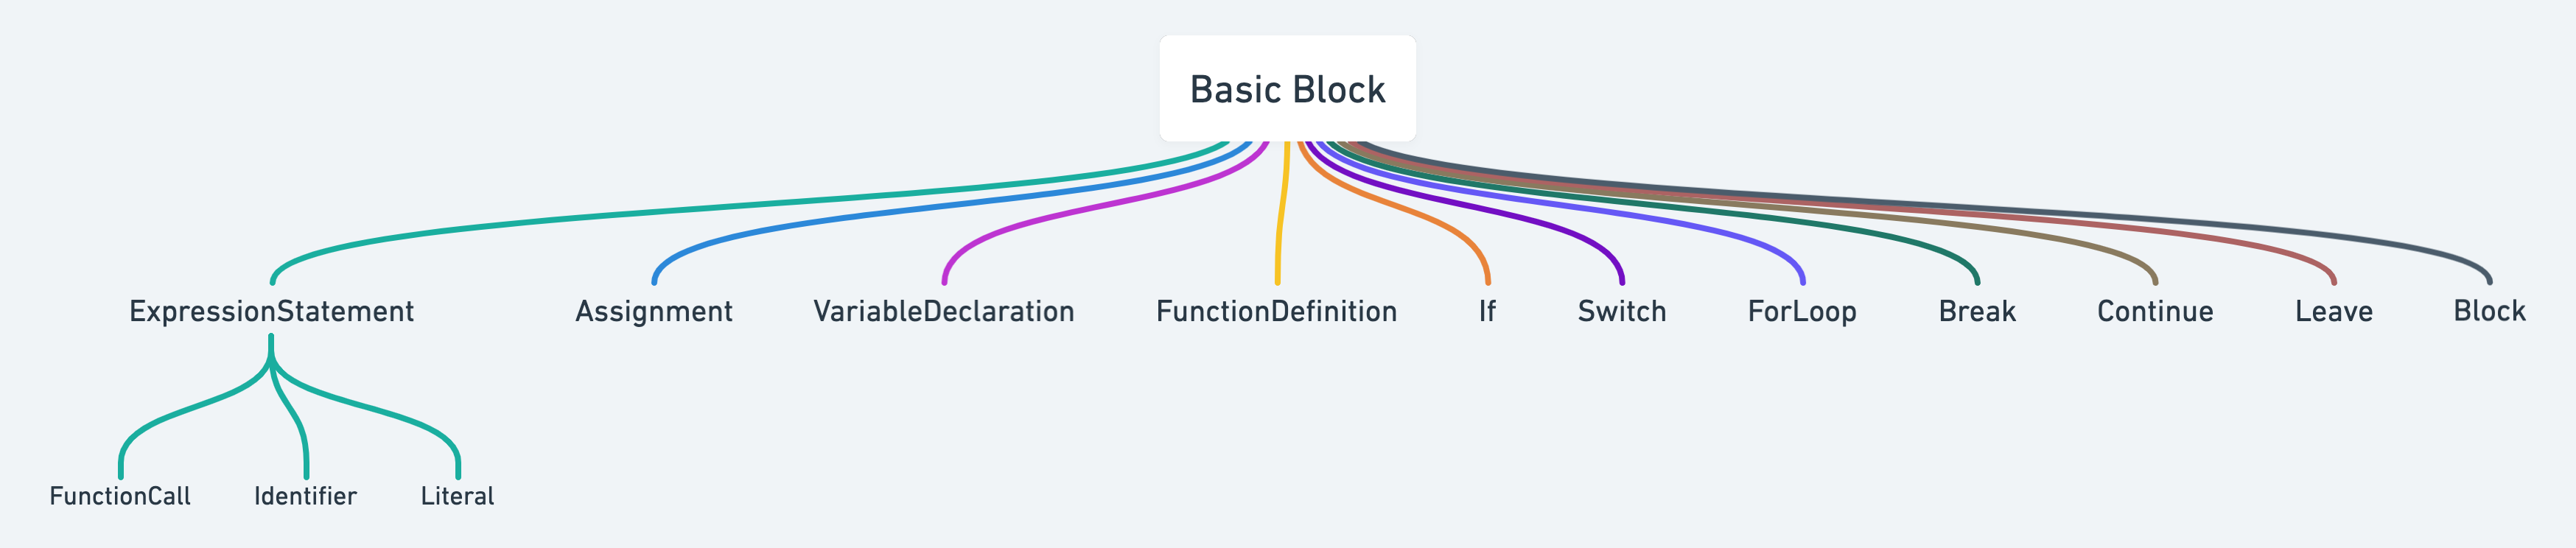
\includegraphics[width=\textwidth]{images/yul_ast_node_types.png}
    \caption{Node types in the YUL AST. Node properties vary depending on their nature.}
    \label{fig:yul-ast-node-types}
\end{figure}


\section{Other tools performing static analysis}
\paragraph*{}
The compiler has the option of outputting the Solidity AST in JSON format, which means that external tools can be built to alter the AST in any desired way. Since the compiler also supports receiving an AST as input, and generate bytecode from that one, that means that in theory one could build a better optimizer than the official one. While that hasn't happened yet, there are a few tools that perform code analysis of their own.

\subsection{Solidity Instrumentation Framework (SIF)}

Built by Chao Peng, Sefa Akca and Ajitha Rajan, from University of Edinburgh, SIF is a tool built in C that gravitates around the Visitor Design Pattern. The main objective is to build an internal C representation of Solidity code, through intermediary data structures, upon which SIF can orchestrate various optimizations / refactoring functions. As the authors describe it, it's a tool \cite[to easily and effectively understand, manipulate and analyse Solidity code]{sif}.

\begin{figure}
    \centering
    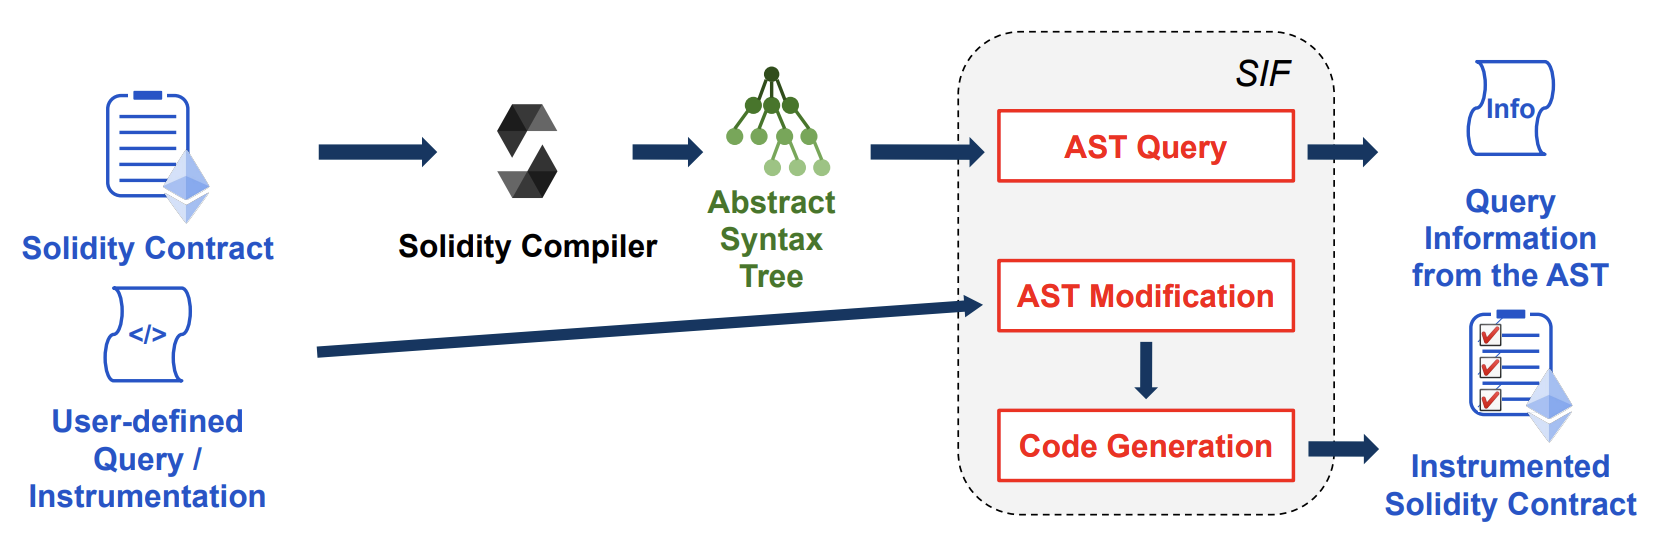
\includegraphics[width=15cm]{images/sif_workflow.png}
    \caption{SIF workflow, captured from SIF: A Framework for Solidity Contract Instrumentation and Analysis \cite{sif}}
    \label{fig:sif-workflow}
\end{figure}

The drawbacks that this toolkit currently has is that it's outdated and that it does not allow for external users to "plug-in" their own intermediate representations of Solidity code. It acts more as a middle-man, allowing users to implement, through the \emph{visit} method, specific optimization / refactoring items that run against isolated pieces of code. The tool does build a Control Flow Graph for the code, the one that this thesis will focus on, but it does not specifically use it for any kind of in-house optimization - it is just available to the user for usage. However, the completeness of the internal control flow graph is questionable.

\subsection{Slither}
\paragraph*{}
Slither is a more abstract, high level static analysis framework, which gives a broader overview over the internals of an Ethereum smart contract. Its main focus is centered around 4 areas: security (vulnerability detection), automated code optimization, code analysis and assisted code review, as described in Section 4.1 by the author Margherita Renieri \cite{slither}.

The tool takes advantage of the Abstract Syntax Tree (AST) built by the Solidity Compiler, then passes that through a series of optimization steps: Information Recovery, SlithIR Conversion and Code Analysis.

What's common in both of the tools we've seen is the usage of Abstract Syntax Trees and Control Flow Graphs, as well as building "proprietary" intermediate representation of the input code.

\begin{figure}
    \centering
    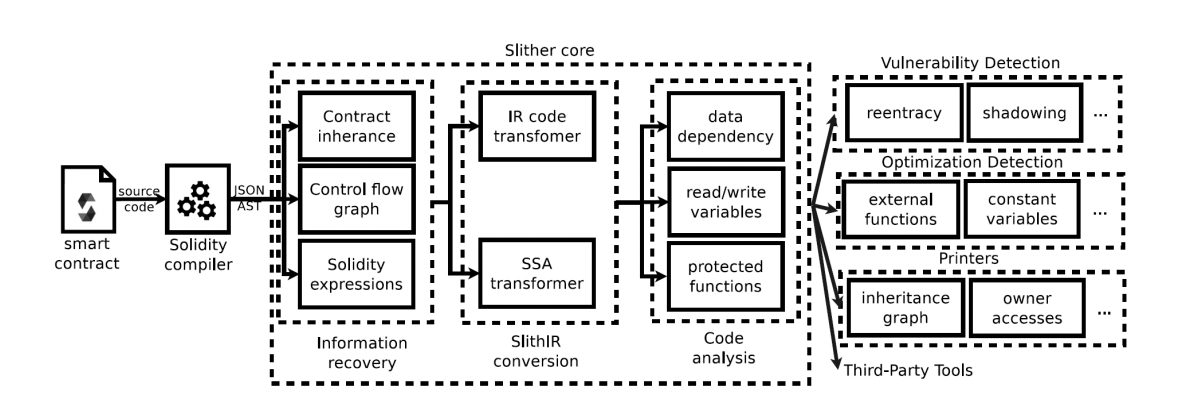
\includegraphics[width=15cm]{images/slither_architecture.png}
    \caption{Slither Architecture}
    \label{fig:slither-architecture}
\end{figure}

\subsection{Why focus on the official optimizer}
\paragraph*{}
The issue with such tools as SIF or Slither is that they get rapidly deprecated, since Solidity ground is so volatile, and they don't provide better optimization flows than Solidity's compiler does. Furthermore, integration is a bit more difficult, since it requires a separate optimization pipeline to be run through this intermediary tools, which just adds an additional burden to generating efficient bytecode.

What is certain is that the official compiler and optimizer will stay at the core of generating the Solidity bytecode. Therefore, any improvements to that will reflect itself in the next Solidity release - given it passes the team's rigurous reviews, of course.
    \chapter{Contributions}

Solidity is a relatively new technology, when compared to already existing programming languages widely used in the market. As stated by the Solidity team itself, "the optimizer is under heavy development" \cite{solidity-optimizer}, which gives plenty of room for contributors to bring their own performance enhancements.

I plan on being one of those contributors, starting from the Solidity code and the AST built by the Solidity compiler itself. I will then evaluate the given inputs and focus on building a specific, low resolution Control Flow Graph, by which memory allocation and cpu cycles can be thoroughly inspected. This would allow for a technical deep dive into the insides of an Ethereum smart contract, which in return can provide useful insights to the user as to how the code can be optimized.

As compared to the other existing tools, this thesis will focus on the latest stable version of Solidity (0.8) and will be built around a set principles focused on scalable, maintainable code analysis tools. Security will also not be the main concern, as there is already plenty of interest in that area.
    
    \chapter*{Draft} 
\addcontentsline{toc}{chapter}{Draft}

\section{Local optimizations}
Optimizing for loops.

\begin{lstlisting}[language=solidity]
// SPDX-License-Identifier: MIT
pragma solidity ^0.8.7;

contract VariableInsideLoop {
    function declareVariableInsideLoop() public pure {
        for (uint i = 1; i <= 1000; i++) {
            uint x = i * i;
        }
    }

    function declareVariableOutsideLoop() public pure {
        uint x;
        for (uint i = 1; i <= 1000; i++) {
            x = i * i;
        }
    }
}
\end{lstlisting}

\^ Compiled with solidity 0.8.7, no optimizations enabled.
inside loop gas cost: 420223 gas
outside loop gas cost: 415250 gas

with 200 optimization runs:
inside loop gas cost: 237215 gas
outside loop gas cost: 232242 gas

Still lower!

\begin{lstlisting}[language=bash]
sergiuiacob@Sergius-MacBook-Pro dataset % solhint variable_declaration_loops.sol

\end{lstlisting}

solhint outputs nothing – it sees no issues

nor does solium (eth lint)


\begin{lstlisting}[language=bash]
sergiuiacob@Sergius-MacBook-Pro dataset % solium -f variable_declaration_loops.sol

No issues found.

sergiuiacob@Sergius-MacBook-Pro dataset % solium -f variable_declaration_if.sol

No issues found.

\end{lstlisting}


variable declaration inside if: 21217 gas
variable declaration outside if: 21274 gas
in this case, outside consumes more gas

200 optimization runs did not change anything

> DISPATCH GAS!!!







TODOs
* test cu persistent var
* TODO ce se intampla daca am acelasi assignment si in outer scope, si in block scope?
* acelasi gen aceeasi_var = aceeasi_val
* pe termination3.sol
  * exemplu ce se intampla cand rulez doar 'Dru'
  * exemplu cum se simplifica si mai mult (datorita static analysis) cand rulez toata suita de optimizatori




Important
* In YUL IR, pot fi instructiuni dupa o instructiune de leave!!!
  * Rezolvat de DeadCodeEliminator
* NU SCOATE assign-ment-urile pentru state variables!!!


Resurse utile
* tips n tricks cu YULs, poate e ceva de folos: https://hackmd.io/@gn56kcRBQc6mOi7LCgbv1g/rJez8O8st
* https://homepages.dcc.ufmg.br/~fernando/classes/dcc888/ementa/
* https://etherscan.io/contractsVerified
  * statistici cu cat \% din contracte folosesc solc 0.8
* tool vizualizare relatii functii din contracte https://piet.blockchains.com/?container=examples%2Fexport1562664060589.piet.json 


De adaugat in teza
* What is Data Flow Analysis?
* function dispatch table <- gas dispatch issue I've had

  * The DataFlowAnalyzer currently does not deal with the ``leave`` statement. This is because
  * it only matters at the end of a function body, which is a point in the code a derived class
  * can not easily deal with.
  ^ Asta scrie in DataFlowAnalyzer.h
* am folosit truffle framework pentru a calcula gas usage-ul in experimentele mele (care ele este doar 1)
* toate variantele pe care le poate lua un assignment


De adaugat in prezentare
* Solidity Summit 2022 – merge la bibliografie I guess.
* https://meet.ethereum.org/solidity – asking questions here. How to make a difference?
* Scheme
  * optimization pipeline (cod solidity -> YUL IR -> YUL optimizer -> EVM Bytecode -> EVM Optimizer (LLVM???) -> bytecode)
* Ce este un dialect. Despre EVM Dialect (folosit de Yul IR)
* cum functioneaza UAE: in documentatie scrie https://docs.soliditylang.org/en/v0.8.14/internals/optimizer.html#redundantassigneliminator
* Despre ce e un AST. Solidity foloseste ANTLR – https://medium.com/@obernardovieira/why-is-ast-so-important-b1e7d6c29260
Proces dezvoltare dizertatie
* Problema: se lucra deja la multe dintre contributiile pe care le consideram sa le fac in solidity de persoane random. trebuia sa gasesc un "free slot" la lucrat la ceva
* Cat de mult ajuta UAE? Experiment cu deployment pt un contract, o functie simpla. Cu si fara optimizarea UAE. DOAR CU ACEEEA!!! Cat gaz se salveaza?
* Am vrut sa imbunatatesc UAE pe AST-ul de pe Solidity – dar dupa o discutie cu echipa Solidity, mi-au clarificat ca optimizarile ar trebui facute pe YUL IR – care are si el un AST, doar ca nu e outputted, e in code base ---> mai dificil
* https://citeseerx.ist.psu.edu/viewdoc/download?doi=10.1.1.453.4245&rep=rep1&type=pdf 
* Fuzzing tests – trying to break the compiler with Etherscan
* default optimization suite de fapt nu e aia prezentata in documentatie – e outdated
  * 'dhfoDgvulfnTUtnIf[xa[r]EscLMcCTUtTOntnfDIulLculVcul [j]Tpeulxa[rul]xa[r]cLgvifCTUca[r]LSsTFOtfDnca[r]Iulc]jmul[jul] VcTOcul jmul'
  * asta pare sa fie... printre altele

Random stuff
  * https://hrkrshnn.com/ prezentari
  * despre patterns care sunt costly dpdv al gazului https://computerscience.unicam.it/marcantoni/tesi/Ethereum%20Smart%20Contracts%20Optimization.pdf
  * despre completeness / corectness CFG https://eprints.ucm.es/id/eprint/61812/1/HERNANDEZ_CEREZO_Tecnicas_de_analisis_para_contratos_inteligentes_generacion_de_grafos_de_control_de_flujo_completos_4398577_720285146.pdf
  * SIF: https://arxiv.org/pdf/1905.01659.pdf
  * basic blocks, etc https://homepages.dcc.ufmg.br/~fernando/classes/dcc888/ementa/slides/ControlFlowGraphs.pdf
  * dispatch gas difference (ce m-a indus pe mine in eroare) slide 11 din https://hrkrshnn.com/t/devconnect.pdf
    * tot intr-una din prezentarile de aici zice ca "opcode optimization should be kept as simple as possible – engineering decision)
  * detaliu: Ethereum blockchain only stores EVM bytecode, so the high level code needs to be optimized before turned into EVM, of course
  * https://eprints.ucm.es/id/eprint/61812/1/HERNANDEZ_CEREZO_Tecnicas_de_analisis_para_contratos_inteligentes_generacion_de_grafos_de_control_de_flujo_completos_4398577_720285146.pdf     <------------- tool care imbunatateste Oyente / EthIR si gaseste security flaws. poate fi aplicat pe codul pe care il generez eu
  * optimizer passes (etape): pot fi platform independent / dependent
  * optimizari facute pe baza YUL, example: function inlining https://www.youtube.com/watch?v=VH4MgZDyZJU&ab_channel=EthereumFoundation
  * despre cum CFG-urile sunt folosite: "Gastap is one of the few tools based on static analysis that manages to infer gas upper
  bounds for transactions. Gastap is one of the most accurate tools in the field, having a
  great success rate. It generates a Control-Flow-Graph (CFG) as an intermediate representation of the analysis. However, the current algorithm used by Gastap is not precise.
  Therefore, a considerable number of smart contracts cannot be analyzed." din https://eprints.ucm.es/id/eprint/61812/1/HERNANDEZ_CEREZO_Tecnicas_de_analisis_para_contratos_inteligentes_generacion_de_grafos_de_control_de_flujo_completos_4398577_720285146.pdf
  * alte moduri in care lumea interpreteaza cod solidity, ex asta cu XML-uri ca sa foloseasca query-uri XPath apoi https://orbilu.uni.lu/bitstream/10993/35862/3/smartcheck-paper.pdf



Misc stuff
* adaugat screenshot cu llvm-opt --help (optimizarile pe care le poate face)
* de vorbit despre ce e "--optimize-runs" (scrie in doc oficial). trade off intre code size / code efficiency
* Simple Inlining a fost adaugat in solidity 0.8.2!!! super recent
* YUL optimizer: "The optimizer currently follows a purely greedy strategy and does not do any backtracking."
* Issues gasite in timp ce lucram la dizertatie
  * cand se construieste AST (--ast-compact-json), la pgrama valoarea pentru "src" nu e corecta, gen de unde pana unde tine codul pt pragma directive
* de folosit un tool online si de aratat cum functioneaza UAE (solc --optimize --ir-optimized --via-ir --yul-optimizations 'r'  termination.sol | pbcopy), o data cu '' si o data cu 'r'    –   https://text-compare.com/

Proprietati noduri CFG
* The	flow	of	control	can	only	
enter	the	basic	block	through	
the	first	instruction	in	the	
block.

Proprietati pentru solidity optimizer (on YUL)
* Disambiguatorul seteaza unique names pt fiecare functie / variabila
* loop related optimizations
  * stop condition is moved into the loop body
  * loop initialization body is moved before the loop
  * majoritatea optimizarilor listate in documentatia oficiala (0.8.14) graviteaza in jurul precalcularii constantelor si propagarii acestora

----din https://homepages.dcc.ufmg.br/~fernando/classes/dcc888/ementa/slides/ControlFlowGraphs.pdf

* first instruction of a block == leader (multiple moduri de a identifica leaders)
* basic blocks pot fi construite in functie de leader-ii identificati
  * un basic block incepe la primul leader si se termina la urmatorul leader

Idei cu ce pot face
* CFG intre contracte?
* diferite rezolutii CFG
* vizualizare CFG (graphviz?)
* dead code elimination (https://homepages.dcc.ufmg.br/~fernando/classes/dcc888/ementa/slides/ControlFlowGraphs.pdf)
  * ca pas intr-un CI
* izolarea codului – cred ca daca iau toate variabilele si le izolez (gen ce e folosit intr-un if sa fie definit acolo) etc. atunci o sa consume mai putin gas
* pentru a-mi testa softul: idei in capitolul 8.1 din https://eprints.ucm.es/id/eprint/61812/1/HERNANDEZ_CEREZO_Tecnicas_de_analisis_para_contratos_inteligentes_generacion_de_grafos_de_control_de_flujo_completos_4398577_720285146.pdf
* ma pot intepa in StructuralSimplifier + Dataflow Analyzer deja existente in solc

Optimizari deja facute de solc
* LoopInvariantCodeMotion – ce vreau eu sa fac de fapt https://docs.soliditylang.org/en/v0.8.14/internals/optimizer.html#loopinvariantcodemotion
  * "variable declarations inside conditional branches will not be moved out of the loop" <- posibilitate de improvement
* Local common subexpression eliminator
* citat din doc oficial: "specializes or inlines functions" (probabil on in loc de or)
  * todo aici, de aratat un exemplu pe YUL direct, inlined vs uninlined (--optimize --ir-optimized versus --ir)


Tipuri de optimizari
* local optimizations – in interiorul unui basic block

Pentru prezentare, Proof of Concept:
* programul meu intr-un CI care propune optimizari la PR-uri pentru cod ;)


How does LLVM work? Let's take that for example
* Virtual Register Allocation (ca exemplu)
https://homepages.dcc.ufmg.br/~fernando/classes/dcc888/ementa/slides/ControlFlowGraphs.pdf

    \chapter{Conclusions} 

\paragraph*{}
Optimization is a common process done in compilers that will continue to gain interest from the research and development community. As seen in some of the examples, it can make resource usage even four times lower, while not sacrificing the accessability that high level code brings. Statically typed programming languages usually end up as being preferable in the later phases of program development, as they enforce strict type usage, give little room for interpretation, have an extra layer of security thanks to static analysis (eg. it can automatically detect runtime issues through symbolic execution) and lastly, but definitely not least, generate efficient bytecode thanks to compilers.

\paragraph*{}
Solidity is still a place where "construction is in progress". Thanks to the possibility of external contributions, effective handling of edge cases was implemented directly in the official compiler's codebase, giving seamless integration with the ecosystem. We've managed to have better gas usage for specific smart contracts, while maintaining the corectness of the data flow analysis step. Further work consists in merging the above enhancements through isolated PRs in Solidity's codebase.

    % \chapter*{Bibliography} 
% \addcontentsline{toc}{chapter}{Bibliography}

\begin{thebibliography}{9}
    \bibitem{solidity-documentation} Solidity Official documentation, Solidity Team \url{https://docs.soliditylang.org/en/v0.8.13/internals/optimizer.html#optimizer-steps}
    
    \bibitem{sif} Solidity Instrumentation Framework (SIF), Chao Peng, Sefa Akca, Ajitha Rajan, University of Edinburgh, 2019 \url{https://arxiv.org/pdf/1905.01659.pdf}
\end{thebibliography}
\end{document}
